\documentclass[a4paper,11pt,german,notitlepage]{report}
\usepackage{xcolor}
\usepackage{tabularx}
\usepackage{dclecture}
\usepackage{qrcode}
\usepackage{awesomebox}
\usepackage{circuitikz}
\usepackage[style=german, german=swiss]{csquotes}
\def\farbe{darkgray} %Hier Farbe definieren
\addbibresource{refs.bib}

\ctikzset{
    logic ports=ieee,
    logic ports/scale=0.8,
    logic ports/fill=lightgray
}

\usetikzlibrary{arrows,shapes.gates.logic.US,shapes.gates.logic.IEC,calc,positioning}

\graphicspath{{img/}}

% Extract Exercises

%\usepackage[active, generate=trigonometry_exercises, extract-env={ex}]{extract}
%\begin{extract}
%\usepackage{xcolor}
%\def\farbe{teal}
%\usepackage{dcexercisesnogrid}
%\exercisetrue
%\end{extract}


%%% Fancy Header and Footer
\renewcommand{\headrule}{\vbox to 0pt{\hbox to\headwidth{\color{\farbe}\rule{\headwidth}{1pt}}\vss}}
\pagestyle{fancy} %eigener Seitenstil
\fancyhf{} %alle Kopf- und Fu§zeilenfelder bereinigen
\fancyhead[C]{Informatik - Gymnasium 1. Klasse - Algorithmen Projekt - Mini Schach} %Kopfzeile mitte
%\fancyhead[R]{\includegraphics[width=0.2cm]{x.png}}

\fancyfoot[C]{\thepage}

%\rfoot{\setlength{\unitlength}{1mm}
%\begin{picture}(0,0)
%\put(5,0){\includegraphics{pic\thepage.ps}}
%\end{picture}}


\parskip=.1cm
\parindent=0cm
\linespread{1.5}



\begin{document}

\section*{Beschreibung}
Mini-Schach auf einem 3x3-Feld ist eine stark vereinfachte und kompakte Variante des klassischen Schachspiels.
Die Farben der Felder spielen für dieses Spiel keine Rolle.
Aufgrund des verkleinerten Spielfelds (nur 9 Felder insgesamt) ist das Spiel einfach(er) zu berechnen und kann in ein Planungsproblem überführt werden.
Zur Notation verwenden wir nicht die übliche Schachnotation mit A-H und 1-8, sondern ein Koordinatiensystem mit $x$ und $y$.
$x =$ Spalte (von links nach rechts): $0, 1, 2$
$y =$ Reihe (von unten nach oben): $0, 1, 2$

\begin{figure}[h!]
    \centering
    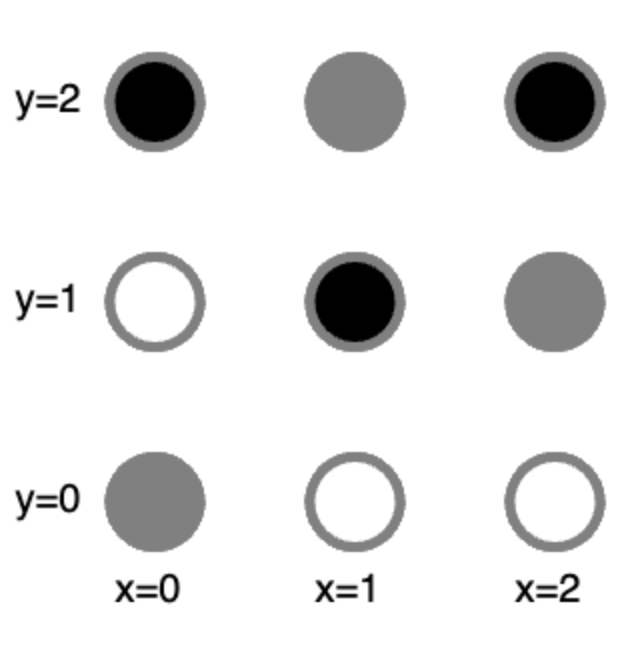
\includegraphics[width=4.5cm]{mini_chess.png}    
    \caption{Screenshot von WebTigerJython. Eine mögliche Spielsituation nach einem Zug. $(0,0) \rightarrow (0,1)$, dann $(1,2) \rightarrow (1,1)$}
\end{figure}

\section*{Regeln}
\begin{description}
    \item[Ziel:] Ein Bauer soll die gegnerische Grundreihe erreichen (Weiss $\rightarrow y = 2$, Schwarz $\rightarrow y = 0$).
    \item[Unentschieden:] Unentschieden, oder Patt wie man im Schach sagt, tritt dann ein, wenn kein legaler Zug mehr möglich ist.
    \item[Züge:] Bauern ziehen ein Feld gerade nach vorne. Weiss also $y + 1$ und Schwarz: $y - 1$. Sie schlagen diagonal nach vorne (z. B. Weiss von $(0,0)$ nach $(1,1)$, wenn dort ein schwarzer Bauer steht). Kein Doppelschritt von der Grundlinie, kein \textit{en passant}.
\end{description}

\section*{Aufgabe}
Hier werden zusätzliche Aufgaben beschrieben, welche spezifisch für Ihr Projekt sind.
Die Aufgaben sind in zwei Gruppen unterzeilt: Pflichtaufgaben und optionale Aufgaben.
Die Pflichtaufgaben sollen am Ende des Projektes beantwortet sein.
Die optionalen Aufgaben dienen dazu, sich weiter im Thema zu vertiefen.
Diese Aufgaben sind Vorschläge. Sie dürfen auch eigene Fragestellungen vertiefen.
Deklarieren Sie Ihre Fragestellungen klar im Projektbericht.
Für alle Projekt gilt natürlich, dass Sie zuerst die allgemeine Aufgabenstellung und den Code (falls vorhanden) verstehen sollten, bevor Sie die untenstehen Aufgaben bearbeiten.
\subsection*{Pflichtaufgaben}
\begin{itemize}
    \item Schreiben Sie einen Minischachcomputer, welcher den zufällig spielenden Computergegner zu mehr als 50\% der Spiele schlägt. Überlegen Sie sich dazu eine Heuristik bei der Auswahl der Züge.
\end{itemize}
\subsection*{Optionale Aufgaben}
\begin{itemize}
    \item Was passiert, wenn Sie die Grösse des Schachbretts verändern? Funktioniert Ihre Heuristik noch? Was müssten Sie ändern und wieso?
    \item Wie ändert sich das Spiel, wenn das Spielbrett mindestens 4x4 Felder gross ist und Sie Doppelzüge von der Grundposition aus erlauben? Funktioniert Ihre Heuristik noch? Wie müssten Sie dazu die Spiellogik im Code ändern?
\end{itemize}

\end{document}  
